\notessection{Mobile Robot Kinematics}
Motion planning and control are fundamental components of robotic autonomy\cite{SiegwartNourbakhshEtAl2011}. For example, in order for an autonomous car to accomplish an objective (e.g. move from point A to B) it first needs to plan a trajectory and determine what control inputs (e.g. throttle and steering) will enable it to follow the trajectory. Both of these components require an understanding of the physical behavior of the robot in order to develop reasonable/actionable plans and controls. In the context of motion planning and control, a robot's physical behavior is generally characterized by its \textit{dynamics} and \textit{kinematics}.

\begin{definition}[Dynamics]
A robot's \textit{dynamics} describe the relationship between forces acting on the robot and changes to the robot's physical state.
\end{definition}
In other words, dynamics can be thought of as the result of Newton's Second Law ($F=ma$) in the context of a particular robot. For example, the dynamics of an autonomous car would describe the relationship between acceleration and forces induced by the tires, gravity, aerodynamics, and so on.

\begin{definition}[Kinematics]
A robot's \textit{kinematics} describe additional restrictions (constraints) on the robot's motion that are \textit{not} induced by forces.
\end{definition}

The most trivial example is that the rate of change of the robot's position must equal its velocity. More generally a robot's kinematics describe limitations on its motion that are a function of the robot's physical state or geometry. For example a robotic arm with multiple joints is kinematically constrained since the rigid connections at each joint only allow rotation about a single axis.

From the preceding descriptions it should be noted that a robot's dynamics and kinematics describe limitations on its motion in different ways\sidenote[][-5\baselineskip]{One simple heuristic for determining how a particular constraint/relationship should be classified is to remember that dynamics are affected by changing the robot's mass, while kinematics are \textit{not}.}.
Not only is it important to identify and describe a robot's dynamics and kinematics, but a roboticist should also ask:
\begin{enumerate}
    \item Do I need to consider \textit{all} of the dynamics/kinematics? Are they all important to the robot's task?
    \item Can any of the dynamics/kinematics be simplified/approximated to make the motion planning and control task easier? 
\end{enumerate}
The combination of dynamics and kinematics make up a \textit{model} of the physical behavior of the robot, and depending on the robot's task some models may be more appropriate than others. In particular the complexity of the model often needs to be balanced with its accuracy/relevance for the task at hand. 

To illustrate this, consider again the autonomous car example. The most accurate model would leverage the car's dynamics, and would include engine dynamics, suspension dynamics, tire dynamics, and so on. In particular, incorporating tire dynamics is critical to understand the phenomenon of drifting, which may be important for motion planning and control in autonomous racing applications. However in other applications it may be more appropriate to simplify the model by replacing the tire \textit{dynamics} with a simple \textit{kinematic} constraint that the tires cannot move laterally (i.e. a ``no side slip'' constraint).

In fact, in the context of motion planning and control for robotics, models built entirely from kinematics can be very useful (and much simpler). For this reason this chapter specifically focuses on robot kinematics, and in particular:
\begin{enumerate}
    \item How to express the configuration of a robot in terms of \textit{general coordinates}
    \item How to mathematically express kinematic constraints in terms of general coordinates
    \item How to identify different types of kinematic constraints, namely \textit{holonomic} and \textit{nonholonomic} constraints
    \item Examples of kinematic models, specifically for wheeled robots
\end{enumerate}


\subsection{Generalized Coordinates}
A robot's physical state (also commonly referred to as its ``configuration'') can usually be represented (i.e. quantified) in different ways. The particular choice of representation defines a finite set of numbers known as \textit{generalized coordinates}.

\begin{definition}[Generalized Coordinates]
Generalized coordinates refer to a set of coordinates that can completely specify the unique position of your robot.
\end{definition}

For example, the wheel rolling on a plane in Figure \ref{fig:non slip disk} can be represented by three parameters, $x, y,\text{and } \theta$, where $(x, y)$ indicates the position at which the wheel touches the ground, and $\theta$ indicates the direction the wheel is traveling in the general frame. This set of parameters $(x,y, \theta)$ that define the wheel's configuration are generalized coordinates for this system. Note that in practice people often use ``configuration'' and ``generalized coordinates'' interchangeably, even though the specific choice of generalized coordinates are not necessarily the only possible representation of the robot's configuration.


The generalized coordinates are mathematically expressed by the vector $\bxi \in \R^n$, where $n$ is the number of generalized coordinates used to describe the robot's configuration.
A robot's motion through time (i.e. its trajectory) is then expressed by the function
\begin{equation*}
    \bxi(t): \R \to \R^n,
\end{equation*}
where $t$ denotes time. In the case of the wheel in Figure \ref{fig:non slip disk} the generalized coordinate vector would be $\bxi = \begin{bmatrix} x & y & \theta \end{bmatrix}^\top $.

\begin{figure*}[ht] 
    \centering 
    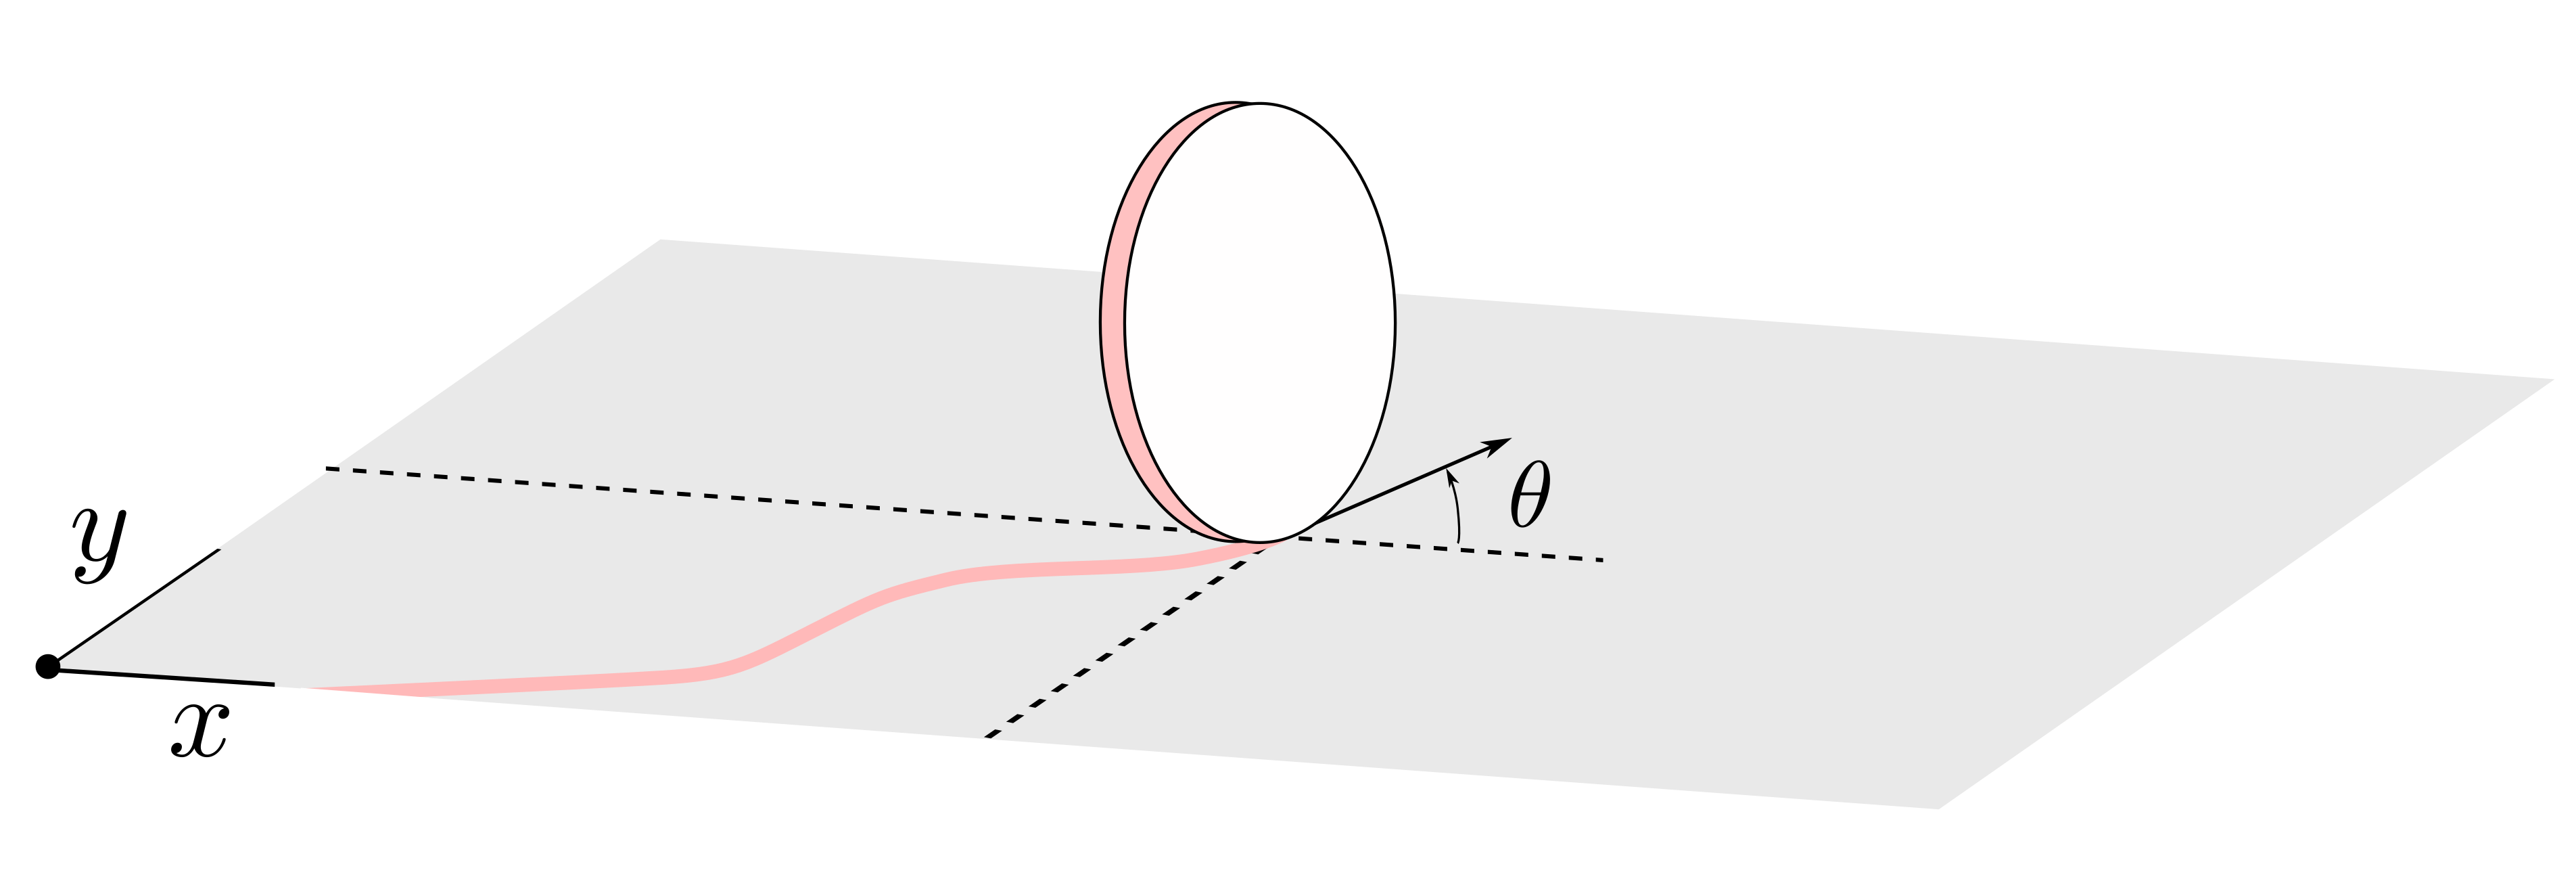
\includegraphics[width=0.65\linewidth]{tex/figs/ch01_figs/wheel_roll.png}
    \caption{Generalized coordinates for a wheel rolling without slipping on a plane.} 
    \label{fig:non slip disk} 
\end{figure*} 

\subsection{Kinematic Constraints}
Once a set of generalized coordinates $\bxi$ has been identified, they can be used to mathematically define kinematic constraints that define a robot's motion. A more formal definition of general kinematic constraints is first presented:

\begin{definition}[Kinematic Constraints]
Let the generalized coordinates of a robot be denoted as $\bxi =[\xi_1, \dots, \xi_n]^\top  $. Constraints that depend on these generalized coordinates and their velocities are called kinematic constraints and are expressed as
\begin{equation} \label{eq:kinconst}
    a_i(\bxi, \dot{\bxi}) = 0, \quad \quad i = 1, \dots, k < n
\end{equation}
where $\dot{\bxi} = \frac{d\bxi}{dt}$ are the velocities.
\end{definition}

Kinematic constraints in robotics applications are often linear with respect to the generalized velocities. Constraints of this kind are referred to as \textit{Pfaffian constraints} and are expressed as
\begin{equation} \label{eq:pfaffian}
    a_i^\top (\bxi)\dot{\bxi} = 0, \quad \quad i =1, \dots, k < n
\end{equation}
where $a_i(\bxi) \in \R^n$. For notational simplicity these constraints can be compactly expressed in matrix form as
\begin{equation}
    A^\top (\bxi)\dot{\bxi}=\bm{0},
\end{equation}
where $A(\bxi) \in \R^{n \times k}$.


\begin{example}[Pendulum] \label{ex:pendulum}
\theoremstyle{definition}
Figure \ref{fig:pendulum} shows a simple pendulum that is assumed to rotate about a fixed pivot point. Let the position of the mass be given by the Cartesian coordinates $(x,y)$, which can be used as the generalized coordinates for this system (i.e. $\bxi = [x, y]^\top $). Since the rod connecting the pivot point to the mass is assumed to be rigid this implies a kinematic constraint. Assuming the pivot point is at the origin $(0,0)$ this constraint can be expressed as
\begin{equation} \label{eq:pendholonomic}
a_1(\bxi) = x^2 + y^2 - L^2 = 0,    
\end{equation}
where $L$ is the length of the rod. Note that while this does not appear to be a Pfaffian constraint, it can be equivalently expressed as one. In particular, consider the derivative of the expression with respect to time, which yields the Pfaffian constraint
\begin{equation} \label{eq:pendpfaffian}
\frac{d a_1(\bxi)}{dt} = \frac{d a_1(\bxi)}{d\bxi}\dot{\bxi} = 2x\dot{x} + 2y\dot{y} = 0,
\end{equation}

In this particular case a more natural choice of coordinates would simply be $\bxi = [\theta]$, which also fully specifies the system's configuration and eliminates the need to enforce additional kinematic constraints. In fact, it can be noted that since $x = L\sin \theta$ and $y = -L \cos \theta$ that the above kinematic constraint is trivially satisfied for all $\theta$.
\end{example}

\begin{marginfigure}
    \centering 
    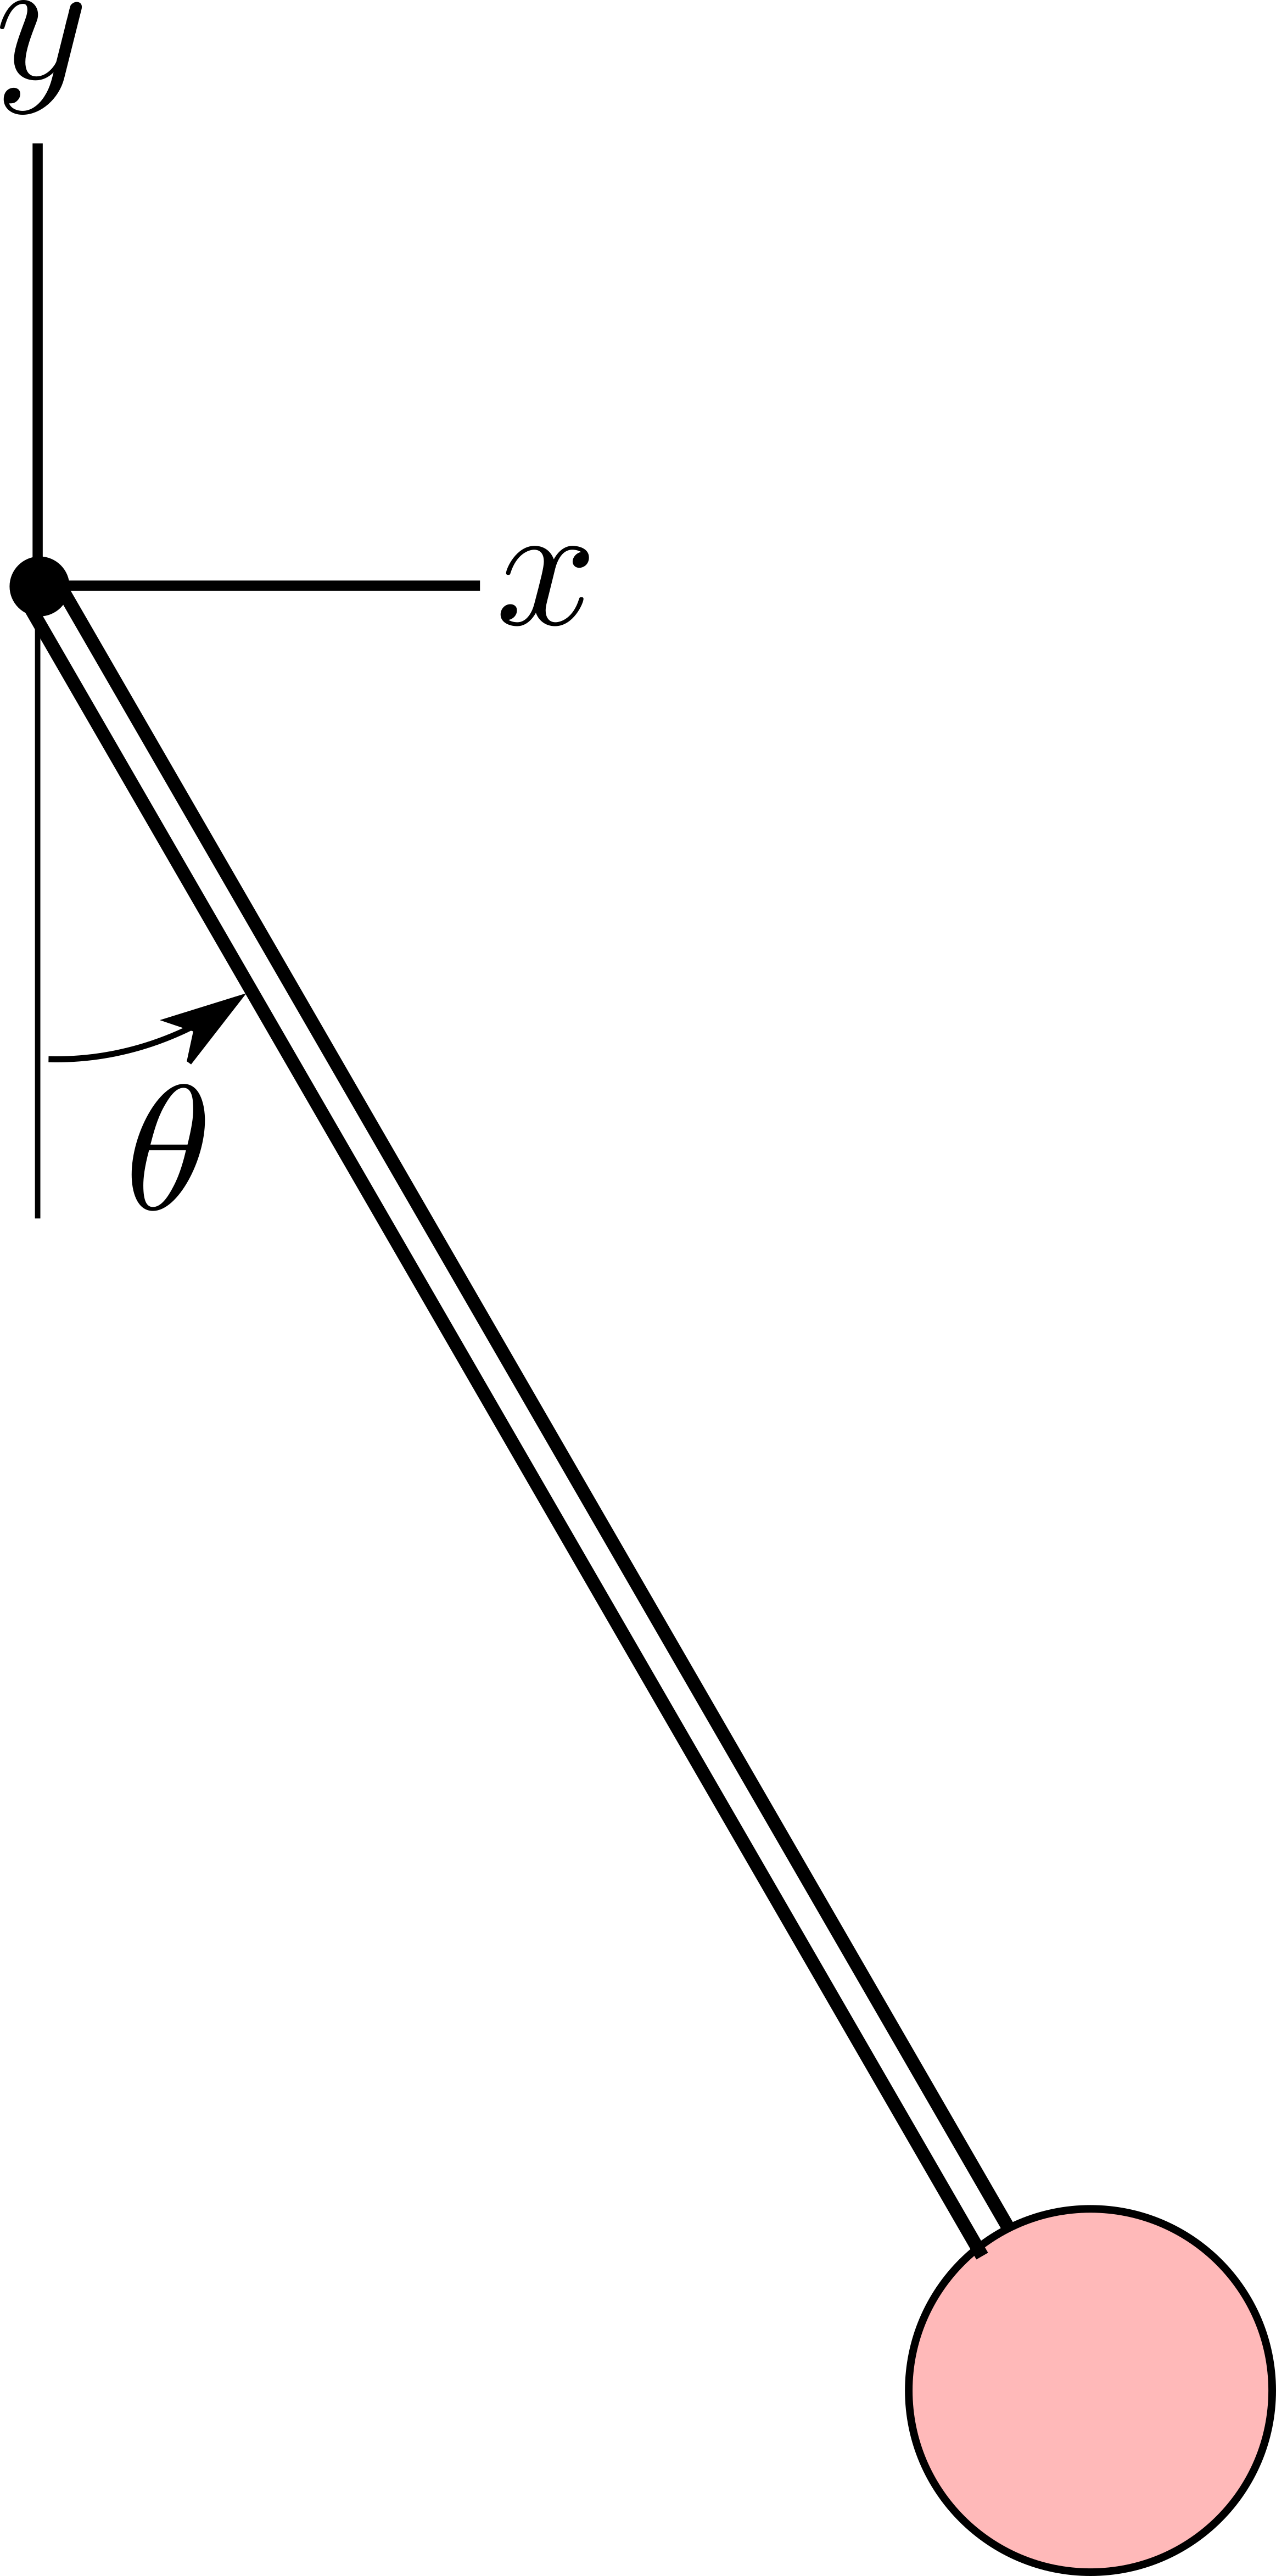
\includegraphics[width=0.55\linewidth]{figs/ch01_figs/pendulum.png}
    \caption{Generalized coordinates for a simple pendulum. } 
    \label{fig:pendulum} 
\end{marginfigure} 



\begin{example}[No-Slip Wheel] \label{ex:noslipwheel}
\theoremstyle{definition}
Consider again the wheel illustrated in Figure \ref{fig:non slip disk} with generalized coordinates $\bxi = [x, y, \theta]^\top $, and assume that there is a no-slip condition between the wheel and the plane it rolls on. This no-slip condition means that the velocity component of the wheel in the lateral direction is always zero. Since the heading of the wheel is given by the unit vector $e_v = [\cos\theta, \:\sin\theta]^\top $, the lateral direction can be described by the perpendicular unit vector $e_{v,\perp} = [\sin\theta, \: -\cos\theta]^\top $. 

Since the velocity vector is $v = [\dot{x}, \: \dot{y}]^\top $, the no-slip kinematic constraint can be expressed by the inner product $v \cdot e_{v,\perp} = 0$, which is equivalently expressed as
\begin{equation} \label{eq:wheelnonholonomic}
a_1(\bxi,\dot{\bxi}) = \dot{x} \sin\theta - \dot{y} \cos \theta = 0.
\end{equation}
Note that this constraint is linear in the generalized velocities $(\dot{x}, \dot{y})$ and therefore is a Pfaffian constraint.
\end{example}


\subsection{Holonomic and Nonholonomic Constraints}
It is useful to further classify different types of kinematic constraints based on how they restrict the motion of the system. In particular, the most common classifications for kinematic constraints are \textit{holonomic} or \textit{nonholonomic}.

\subsubsection{Holonomic Constraints}
Holonomic constraints are kinematic constraints that can be expressed as a function of \textit{only} the generalized coordinates (without dependence on generalized velocities).
In robotics applications, holonomic constraints generally arise due to mechanical interconnections, such as rigid links and joints of a robotic arm.

\begin{definition} [Holonomic Constraints]
Constraints that can be expressed in the form 
\begin{equation}
    h_i(\bxi) = 0, \quad i = 1, \dots, k < n
    \label{eq:holonomic}
\end{equation}
are called holonomic.
\end{definition}
Additionally, a \textit{holonomic system} is a system that is only subject to holonomic constraints.
Note that these constraints can \textit{always} be equivalently expressed as Pfaffian constraints of the form \eqref{eq:pfaffian} by differentiating the expression
\begin{equation}
\frac{dh_i(\bxi)}{dt} = \frac{dh_i(\bxi)}{d\bxi}\dot{\bxi} = a_i^\top (\bxi) \dot{\bxi} = 0. \quad i = 1, \dots, k < n
\end{equation}
However, it is important to note that not all Pfaffian constraints are holonomic. A Pfaffian constraint is only holonomic if it is \textit{integrable} to the form \eqref{eq:holonomic}.

Holonomic constraints are a unique subclass of kinematic constraints that \textit{restrict the accessible configurations of the system}. In fact, the space of accessible configurations for a system with $n$ generalized coordinates under $k$ holonomic constraints will have dimension $n-k$.

\paragraph{Examples:}
Consider again the pendulum from Example \ref{ex:pendulum}, where the kinematic constraint \eqref{eq:pendholonomic} can be expressed as $h_i(\bxi) = 0$ (equivalently where the Pfaffian constraint \eqref{eq:pendpfaffian} is integrable into the form $h_i(\bxi) = 0$). This constraint restricts the pendulum mass to lie on a circle of radius $L$, which is a one dimensional subset ($n-k = 2-1 = 1$). 

Alternatively, consider the wheel from Example \ref{ex:noslipwheel}, where the kinematic constraint \eqref{eq:wheelnonholonomic} \textit{cannot} be integrated to yield a constraint of the form $h_i(\bxi) = 0$. In contrast to the pendulum, this system has no restriction on what configuration it can be in as it can potentially move to any point $(x,y)$.


\subsubsection{Nonholonomic Constraints}
While holonomic constraints are kinematic constraints which restrict the accessible configurations of the system, not all kinematic constraints are holonomic. In particular, it is possible to have kinematic constraints that \textit{do not} restrict accessible configurations, but rather restrict the motion \textit{between} configurations. These constraints are referred to as \textit{nonholonomic} constraints.

\begin{definition} [Nonholonomic Constraints]
Constraints that can be described in Pfaffian form, but cannot be integrated to $h_i(\bxi) = 0 $ form are called nonholonomic.
\end{definition}
Additionally, a \textit{nonholonomic system} is a system that is subject to at least one nonholonomic constraint.
The restriction of instantaneous motion that is induced by a nonholonomic constraint can be interpreted by considering the Pfaffian form $a_i(\bxi)^\top \dot{\bxi} = 0$. It is clear that for any coordinate $\bxi$, this constraint limits the motion ($\dot{\bxi}$) to lie in the null space of $a_i(\bxi)^\top $.

\paragraph{Examples:}
Consider again the wheel example from Example \ref{ex:noslipwheel} which has a nonholonomic constraint
\begin{equation*}
a_i(\bxi)^\top \dot{\bxi} = \begin{bmatrix}
\sin \theta & -\cos \theta & 0
\end{bmatrix}\dot{\bxi}=0.
\end{equation*}
The null space of $a_i(\bxi)^\top $ in this case is spanned by the vectors $[\cos \theta, \: \sin \theta,\: 0]$ and $[0, \: 0,\: 1]$ which suggests that any potential motion must be made up of a linear combination of these vectors. Intuitively this would be expected because $[\cos \theta, \: \sin \theta,\: 0]$ is the unit vector in the direction of rolling, and $0, : 0,\: 1]$ would correspond to the wheel spinning but not rolling. 

\subsection{Kinematic Models}
Once an appropriate set of generalized coordinates $\bxi \in \R^n$ and all relevant kinematic constraints have been identified for a particular robot the next step is to develop a kinematic model.
In particular these kinematic models will consist of a set of differential equations of the form $\dot{\bxi}(t) = G(\bxi(t))\bu(t)$, where $\bu(t)$ is referred to as a system input or \textit{control}. Given a particular input $\bu(t)$ and an initial condition $\bxi(0)$ this model will define a trajectory of the system.

\begin{definition} [Kinematic Model]
Given a generalized coordinate vector $\bxi \in \R^n$ and $k$ Pfaffian kinematic constraints $A^\top (\bxi)\dot{\bxi}=\bm{0}$, a kinematic model can be defined as $\dot{\bxi} = G(\bxi)u$ where the column space of $G(\bxi) \in \R^{n \times n-k}$ spans the null space of $A^\top (\bxi)$. Additionally, for any input $u$ the solutions to the kinematic model are guaranteed to satisfy the Pfaffian constraints.
\end{definition}

Consider $k$ Pfaffian constraints written in matrix form as $A^\top (\bxi)\dot{\bxi}=\bm{0}$ (which can be a combination of holonomic and nonholonomic constraints). As was noted earlier these constraints imply that a generalized velocity $\dot{\bxi}$ is only admissible at a configuration $\bxi$ if it lies in the $n-k$ dimensional null space of the matrix $A^\top (\bxi)$. A new matrix, $G(\bxi) \in \R^{n \times n-k}$ can therefore be defined such that the columns of $G(\bxi)$ span the null space of $A^\top (\bxi)$. In other words, for each column $g_i$ of $G$ it holds that $A^\top (\bxi)g_i = 0$. To ensure that the generalized velocity $\dot{\bxi}$ satisfies the kinematics constraints it is therefore sufficient to require that $\dot{\bxi} = G(\bxi) u$ where $\bu \in \R^{n-k}$ can be \textit{any} vector. To explicitly show why this is true, consider any vector $u$ and write $\dot{\bxi} = G(\bxi)\bu = \sum_{i=1}^{n-k} g_i(\bxi) u_i$. When this is substituted into the Pfaffian constraints the expression becomes
\begin{equation*}
\begin{split}
A^\top (\bxi)\dot{\bxi} &= A^\top (\bxi)\big(\sum_{i=1}^{n-k} g_i(\bxi) u_i\big), \\
&= \sum_{i=1}^{n-k} A^\top (\bxi) g_i(\bxi) u_i, \\
&= 0, \\
\end{split}
\end{equation*}
which shows that the kinematic constraints are satisfied.

\paragraph{Examples:} Consider again the wheel example from Example \ref{ex:noslipwheel} which has a single nonholonomic constraint
\begin{equation*}
a_i(\bxi)^\top \dot{\bxi} = \begin{bmatrix}
\sin \theta & -\cos \theta & 0
\end{bmatrix}\dot{\bxi}=0,
\end{equation*}
where $\bxi = [x,\:y, \:\theta]^\top $. The null space of $a_i(\bxi)^\top $ in this case is spanned by the vectors $[\cos \theta, \: \sin \theta,\: 0]$ and $[0, \: 0,\: 1]$ and therefore the kinematic model is given by
\begin{equation} \label{eq:wheelkinmodel}
\begin{bmatrix}
\dot{x} \\ \dot{y} \\ \dot{\theta}
\end{bmatrix} = \begin{bmatrix}
\cos \theta & 0 \\
\sin\theta & 0 \\
0 & 1
\end{bmatrix}\begin{bmatrix}
u_1 \\ u_2
\end{bmatrix}.
\end{equation}
Note that in many cases the control inputs $u_1$ and $u_2$ also have an intuitive physical meaning. In this problem $u_1$ is the speed at which the wheel is moving, and $u_2$ is the angular rate at which it rotates. 

\subsection{Kinematic Models of Wheeled Robots}
Robots come in all shapes, sizes, and configurations and with varying forms of mobility. However, wheeled robots are perhaps the most widely used because of their high mobility and simple design. For this reason several standard kinematic models for different wheeled robot configurations will now be given.

\subsubsection{Unicycle Model} \label{subsubsec:uni}
The unicycle model of a robot is the simplest kinematic model, and assumes that the robot can be approximated by a single wheel. In this case the kinematic constraints are exactly the same as the wheel rolling on a plane discussed previously in Example \ref{ex:noslipwheel}. A simplified diagram showing the generalized coordinates of this model is given in Figure \ref{fig:uni}, and the kinematic model is the same as \eqref{eq:wheelkinmodel}:
\begin{equation} \label{eq:uni}
\begin{bmatrix}
\dot{x} \\ \dot{y} \\ \dot{\theta}
\end{bmatrix} = \begin{bmatrix}
\cos \theta & 0 \\
\sin\theta & 0 \\
0 & 1
\end{bmatrix}\begin{bmatrix}
v \\ \omega
\end{bmatrix},
\end{equation}
where $v$ is the forward speed of the unicycle and $\omega$ is the rate of rotation.

The advantage of the unicycle model lies in its simplicity and its ability to capture one of the most fundamental behaviors of wheeled robots. Such a model might be suited for higher level motion planning tasks, such as planning geometric paths to get a robot from point A to point B. Often times such a model might be complemented with models of higher fidelity (e.g. dynamics models) for performing lower level tasks such as control or for refining motion plans created by the unicycle model.
\begin{marginfigure}
    \centering 
    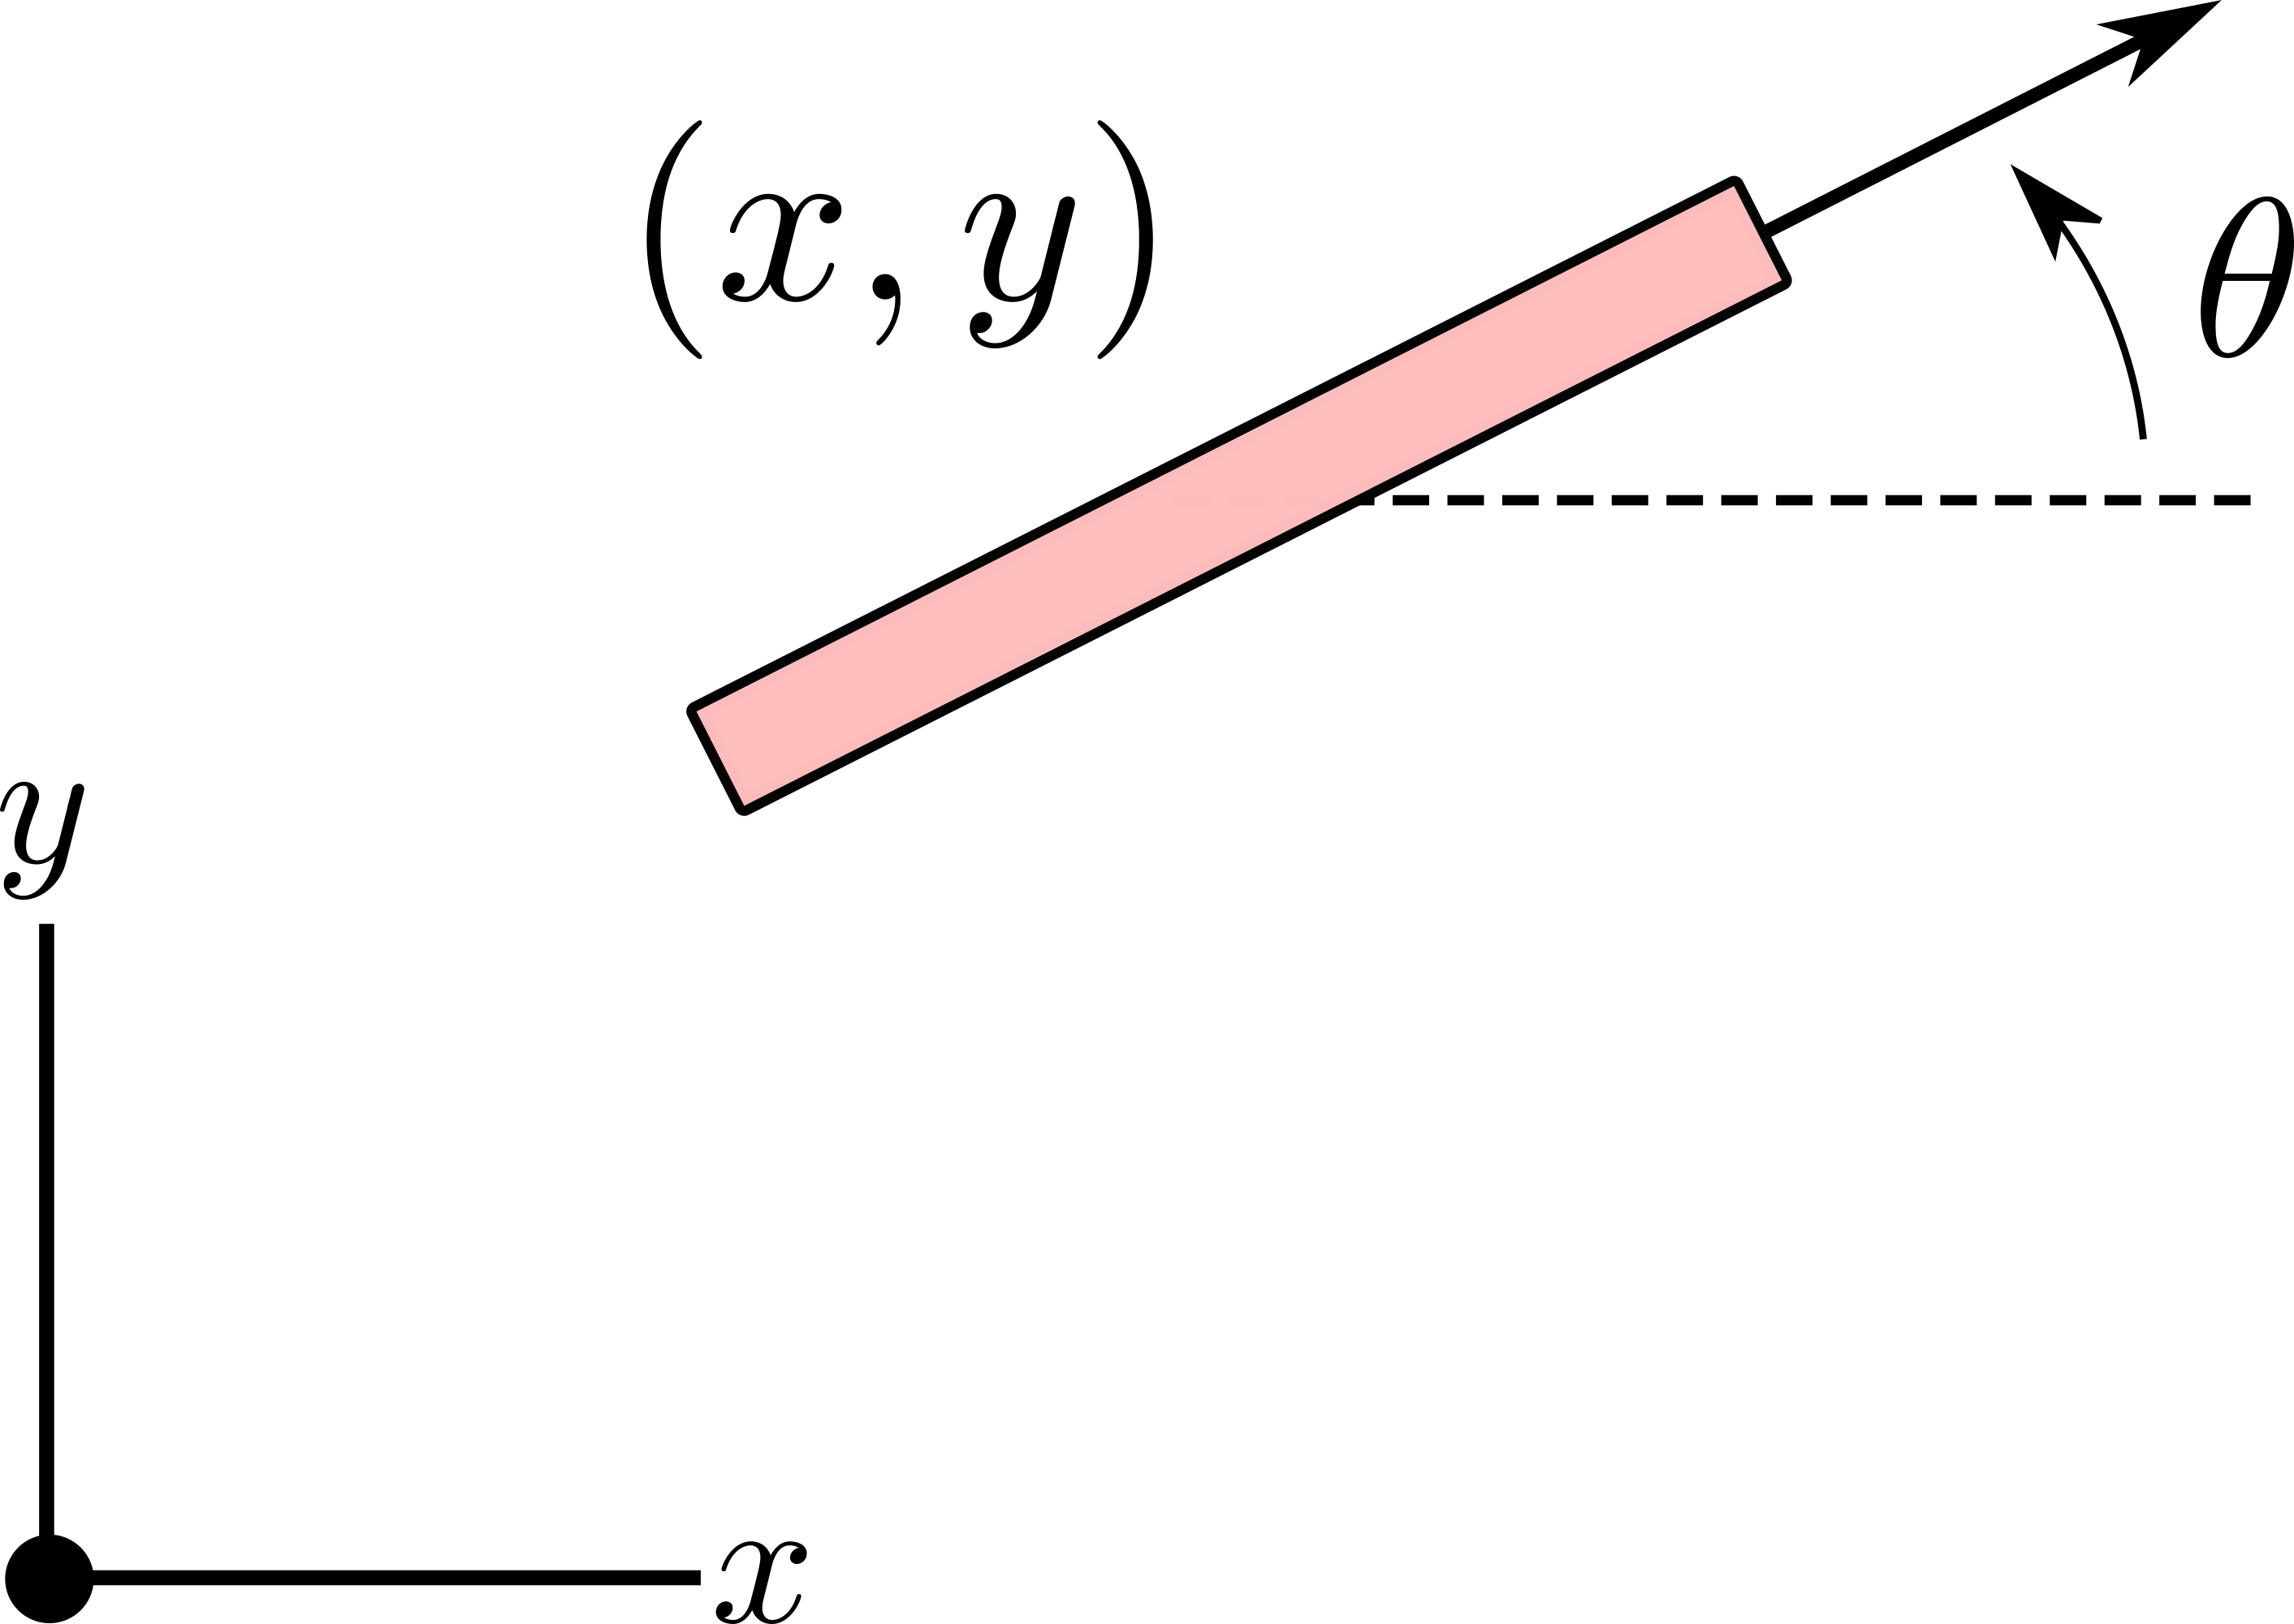
\includegraphics[width=0.8\linewidth]{tex/figs/ch01_figs/unicycle.png}
    \caption{Generalized coordinates for a unicycle.}
    \label{fig:uni} 
\end{marginfigure} 


\subsubsection{Differential Drive Model}
The differential drive model is a slight variation on the unicycle model (see Section \ref{subsubsec:uni}) that does not lump all of the wheels together. Instead, this model assumes two wheels are fixed on a rear shared axle, with a passive wheel that induces no kinematic constraints in the front.
As shown in Figure \ref{fig:dd} this model has the same generalized coordinates as the unicycle model ($\bxi = [x,\:y,\:\theta]^\top $) but also includes some geometry of the robot by assuming the width of the rear axle is denoted by $L$.

Same as for the unicycle model, this model assumes the wheels roll without slipping. The derivation of the kinematic constraints is therefore similar to Example \ref{ex:noslipwheel}. In particular, the heading of each wheel is always given by $e_v = [\cos \theta, \: \sin \theta]^\top $, the lateral direction is given by $e_{v,\perp} = [\sin \theta, \: -\cos \theta]^\top $, and thus the two no-slip kinematic constraints can be expressed as
\begin{equation*}
\dot{p}_l \cdot e_{v,\perp} = 0, \quad \dot{p}_r \cdot e_{v,\perp} = 0,
\end{equation*}
where $\dot{p}_l$ and $\dot{p}_r$ are the left and right wheel velocity vectors, respectively. The next step is to determine how to express $\dot{p}_l$ and $\dot{p}_r$ as functions of the generalized coordinates and generalized velocities. From the geometry of the robot it can be seen that
\begin{equation*}
p_l = [x - \frac{L}{2}\sin \theta, \: y + \frac{L}{2}\cos \theta], \quad p_r = [x + \frac{L}{2}\sin \theta, \: y - \frac{L}{2}\cos \theta],
\end{equation*}
where $p_l$ and $p_r$ are the positions of the left and right wheels. By taking the derivative with respect to time the velocities are given by
\begin{equation*}
\dot{p}_l = [\dot{x} - \dot{\theta}\frac{L}{2}\cos \theta, \: \dot{y} - \dot{\theta}\frac{L}{2}\sin \theta], \quad \dot{p}_r = [\dot{x} + \dot{\theta}\frac{L}{2}\cos \theta, \: \dot{y} + \dot{\theta}\frac{L}{2}\sin \theta].
\end{equation*}
It turns out that after some algebraic manipulation the no-slip kinematic constraints simply become:
\begin{equation*}
\dot{p}_l \cdot e_{v,\perp} = \dot{p}_r \cdot e_{v,\perp} = \dot{x}\sin \theta - \dot{y} \cos \theta = 0,
\end{equation*}
which means having the no-slip kinematic constraint on both wheels is actually redundant! This also makes intuitive sense because the wheels are rigidly connected together, so if one wheel cannot move laterally then the other must not be able to. Additionally, it is noted that this nonholonomic constraint is identical to the one for the unicycle and so the kinematic model is also identical to \eqref{eq:uni}. However the difference is that the \textit{control inputs} can now be expressed in a more realistic form with respect to the actual geometry of the robot.

In particular, instead of the inputs being the forward speed $v$ and body rotation rate $\omega$ as in \eqref{eq:uni}, the inputs will be chosen to be the left and right wheel rotation rates, $\omega_l$ and $\omega_r$. A relationship between these sets of inputs can be derived by exploiting the geometry of the robot and the no-slip wheel assumption. In particular, since the position $p = [x, \: y]$ can be written as $p = \frac{1}{2}(p_l + p_r)$ the velocity vector $\dot{p} = \frac{1}{2}(\dot{p}_l + \dot{p}_r)$. From the no-slip wheel assumption the speed can be expressed as $v = e_v \cdot \dot{p}$, which can be simplified to
\begin{equation*}
\begin{split}
v &= e_v \cdot \dot{p}, \\
&= e_v \cdot \frac{1}{2}(\dot{p}_l + \dot{p}_r), \\
&= \frac{1}{2}(e_v \cdot \dot{p}_l + e_v \cdot \dot{p}_r), \\
&= \frac{1}{2}(v_l + v_r), \\
&= \frac{r}{2}(\omega_l + \omega_r), \\
\end{split}
\end{equation*}
where $r$ is the radius of the wheel and $v_l$ and $v_r$ are the speeds of the left and right wheels. 

Additionally, the no-slip condition on each individual wheel can be expressed as $v_l = e_v \cdot \dot{p}_l$ and $v_r = e_v \cdot \dot{p}_r$ which can be expanded to
\begin{equation*}
\begin{split}
\dot{x}\cos{\theta} + \dot{y}\sin{\theta} - \dot{\theta} \frac{L}{2} &= v_l, \\
\dot{x}\cos{\theta} + \dot{y}\sin{\theta} + \dot{\theta} \frac{L}{2} &= v_r. \\
\end{split}
\end{equation*}
Noting that $\dot{x}\cos{\theta} + \dot{y}\sin{\theta} = v$ these expressions can be written as $\frac{L}{2}\dot{\theta} = v_r - v$ and $\frac{L}{2}\dot{\theta} = v - v_l$. Finally, combining these expressions yields
\begin{equation*}
\begin{split}
L\dot{\theta} &= v_r - v_l, \\
&= r(\omega_r - \omega_l). \\
\end{split}
\end{equation*}
In summary, a one-to-one mapping between the inputs is given by
\begin{equation*}
v = \frac{r}{2}(\omega_l + \omega_r), \quad \omega = \frac{r}{L}(\omega_r - \omega_l).
\end{equation*}
Finally, the differential drive kinematic model is given by
\begin{equation} \label{eq:dd}
\begin{bmatrix}
\dot{x} \\ \dot{y} \\ \dot{\theta} 
\end{bmatrix}
 = 
 \begin{bmatrix}
\frac{r}{2}\cos\theta & \frac{r}{2}\cos\theta \\ 
\frac{r}{2}\sin\theta & \frac{r}{2}\sin\theta \\ 
\frac{r}{L} & -\frac{r}{L}
\end{bmatrix}
\begin{bmatrix}
\omega_r \\ \omega_l
\end{bmatrix}.
\end{equation}

Overall, the complexity of this model over the unicycle model has not increased. However, by leveraging the geometry of the robot the inputs to this model may be more intuitive for motion planning and control tasks since the actual control mechanism is generally a motor attached to the wheel axles. 

\begin{marginfigure}
    \centering 
    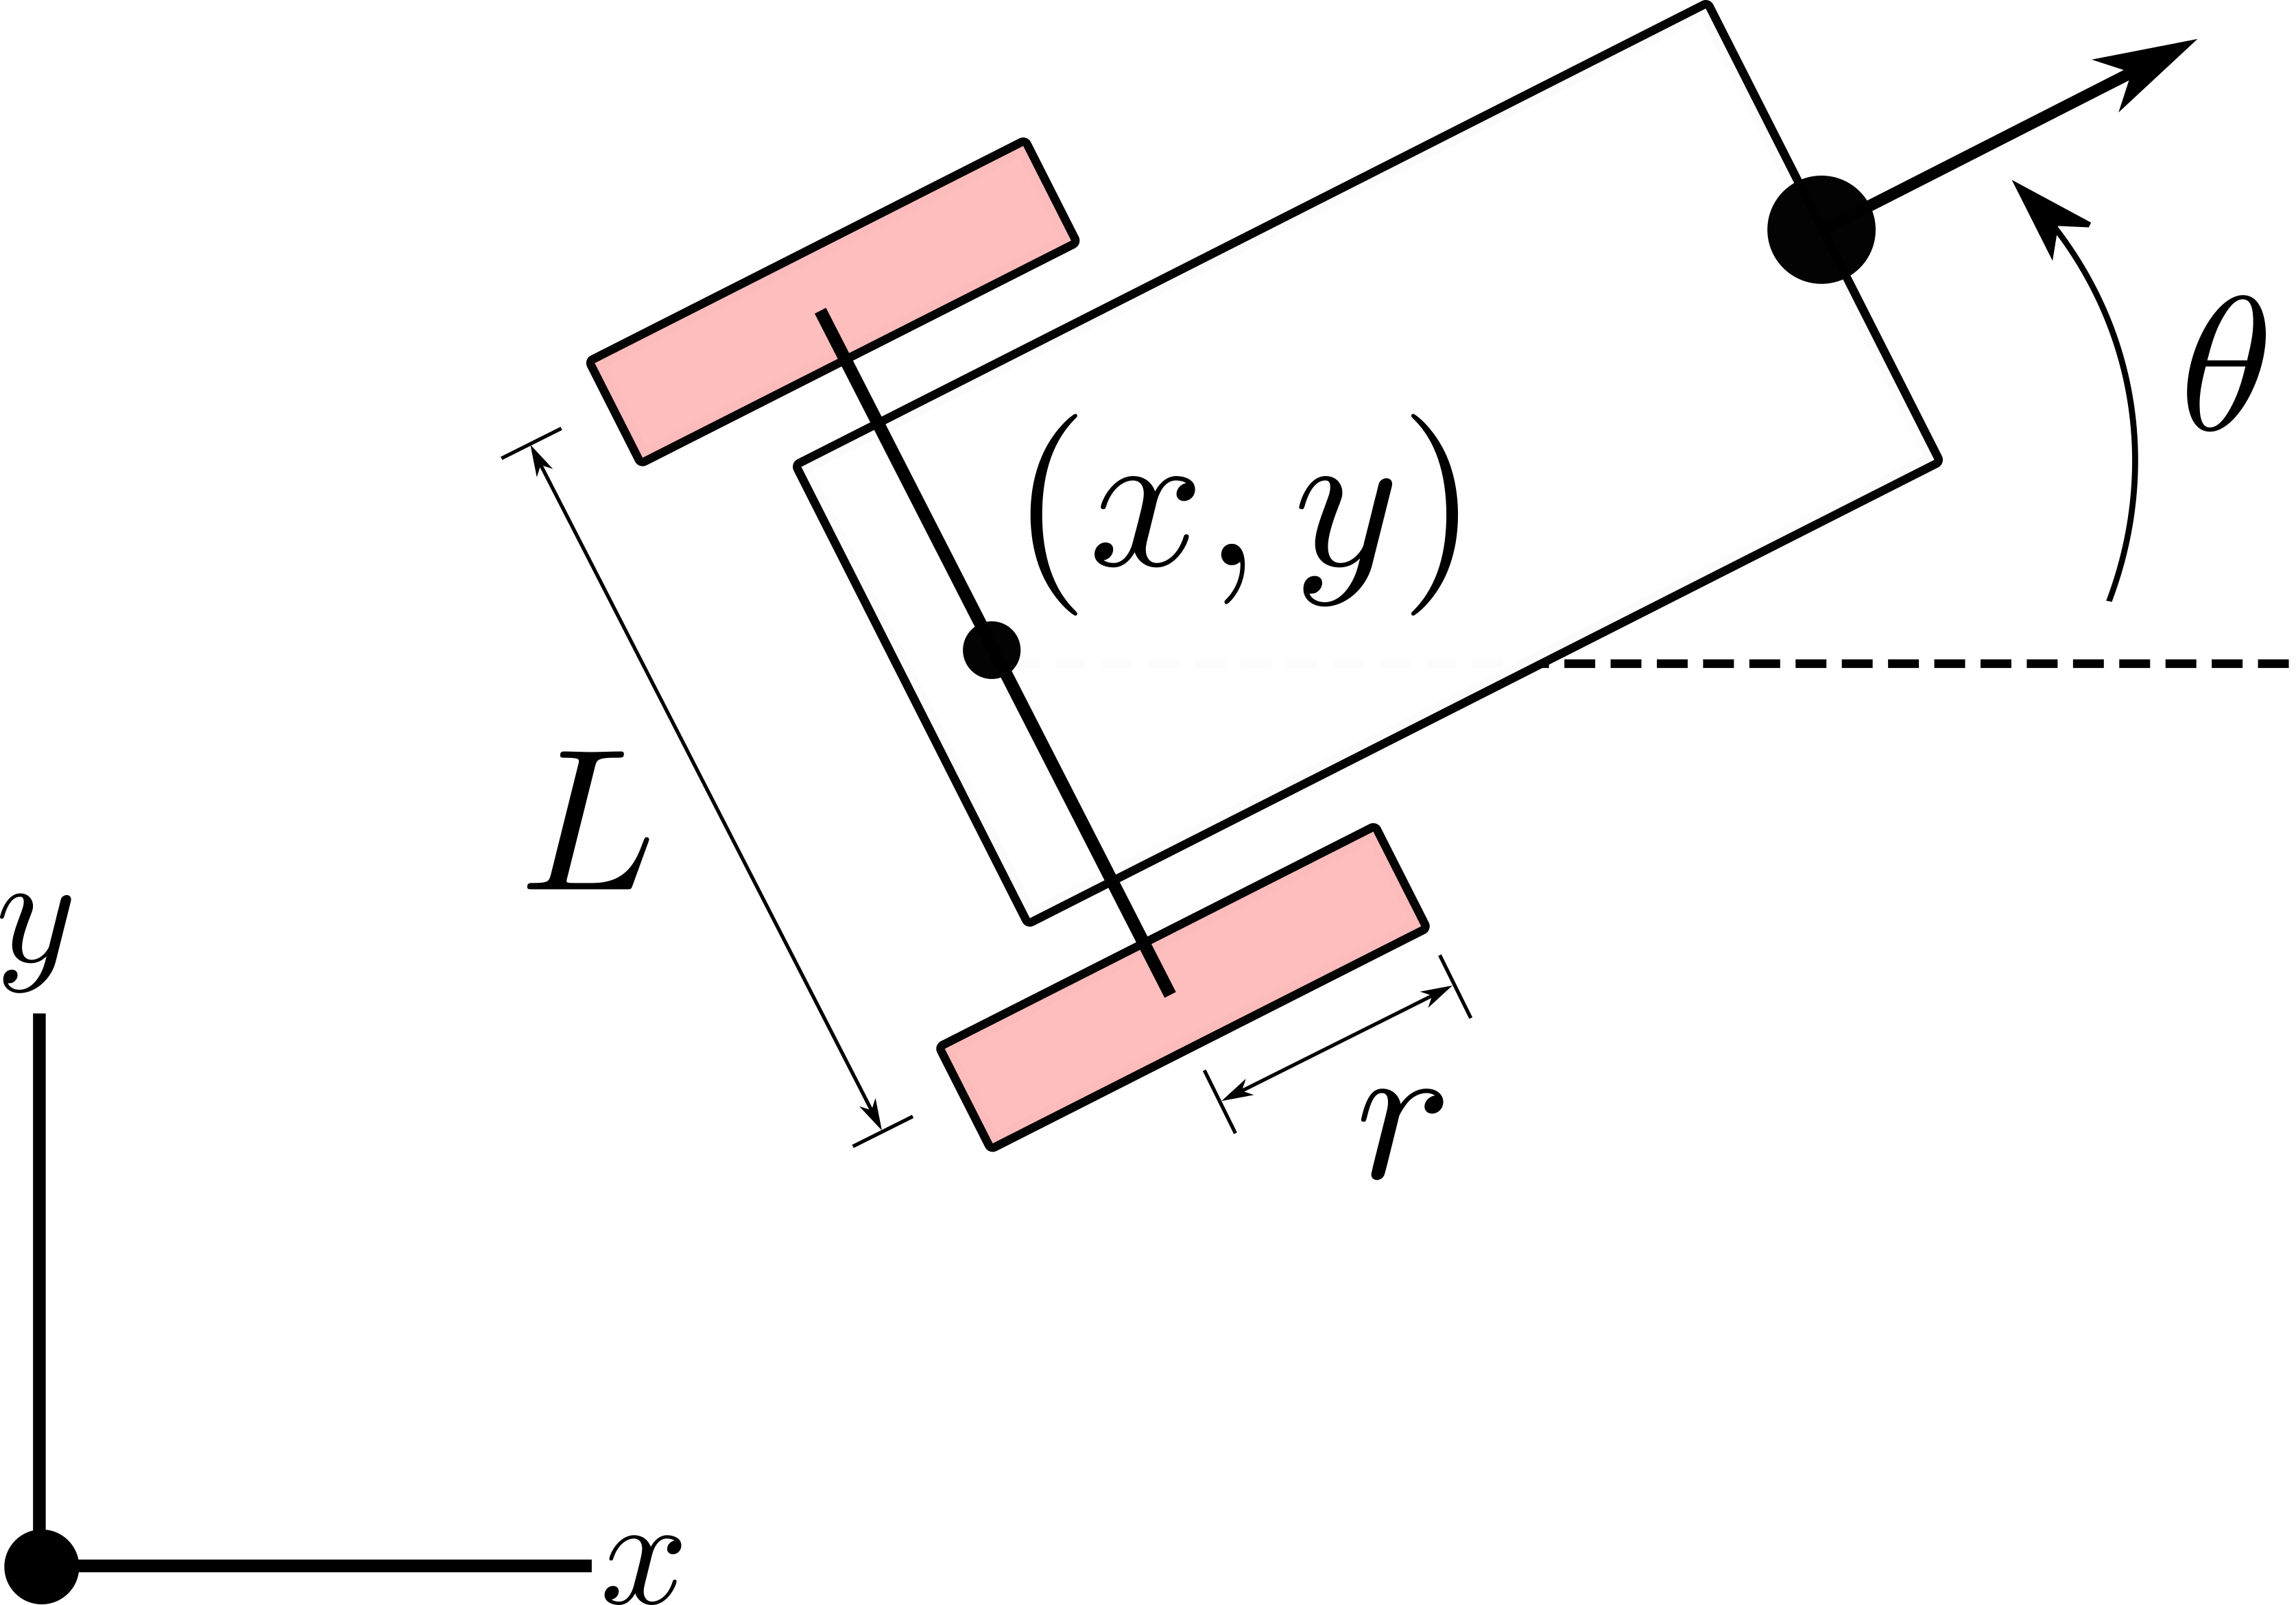
\includegraphics[width=0.9\linewidth]{tex/figs/ch01_figs/diff_drive.png}
    \caption{Generalized coordinates for a differential drive robot.} 
    \label{fig:dd} 
\end{marginfigure} 


\subsection{Dynamic Models}
As was discussed in the introduction, mobile robot kinematic models are useful for describing fundamental physical behavior in a simple way, but they do not \textit{completely} capture all real world influences on the robot's motion. The unicycle and differential drive models are examples of kinematic models that are approximations of the true system behavior. In particular they both make the no-slip wheel assumption, which directly lead to the kinematic constraints. Additionally, the choice of the inputs for the kinematic models ignores other important dynamics of the robot. In the unicycle model it is assumed the velocity is the input, but in practice directly commanding a desired velocity is not always straightforward since the amount of force required to change velocities varies with the mass of the robot ($F=ma$). In the differential drive model the inputs are the rotational rates of the wheels, but again in practice the amount of torque output required by the motor to change the rotation rate can vary depending on the robot's mass as well as other motor dynamics.

One common extension to kinematic models to incorporate \textit{dynamics} is to simply add integrators to replace the input variables. The most common example of this is to replace a velocity input $v$ with an acceleration input $a$ and add the integrator $\dot{v} = a$. The force that generates the acceleration can then be considered as the input by using the dynamics equation $\dot{v} = \frac{1}{m}F$ where $m$ is the mass of the robot. Similarly, a rotation rate input $\omega$ could be replaced by a rotational acceleration input. For example, the unicycle model \eqref{eq:uni} could be extended with integrator states to be
\begin{equation} \label{eq:extendeduni}
\begin{bmatrix}
\dot{x} \\ \dot{y} \\ \dot{v} \\ \dot{\theta}  \\ \dot{\omega}
\end{bmatrix} = \begin{bmatrix}
v\cos \theta  \\
v\sin\theta \\
a \\
\omega \\
\alpha
\end{bmatrix}.
\end{equation}
where $a$ is linear acceleration in the forward direction and $\alpha$ is the angular acceleration (which of course could also be written with forces and torques as inputs).

In summary, factors to consider when deciding whether a certain kinematic model is sufficient. or if additional kinematics/dynamics are needed. include the robot's configuration/geometry and the task at hand (e.g. planning, control, etc.).